
\chapter{Simulator}
\label{chap:simulator}
\section{Description}


At the beginning of this project, we had at our disposal the simulator of Mr Teodorov (figure \ref{fig:sim}). This simulator have a graphic user interface as you can see on the figure \ref{fig:sim}.


\begin{figure}[h]
  \centering
  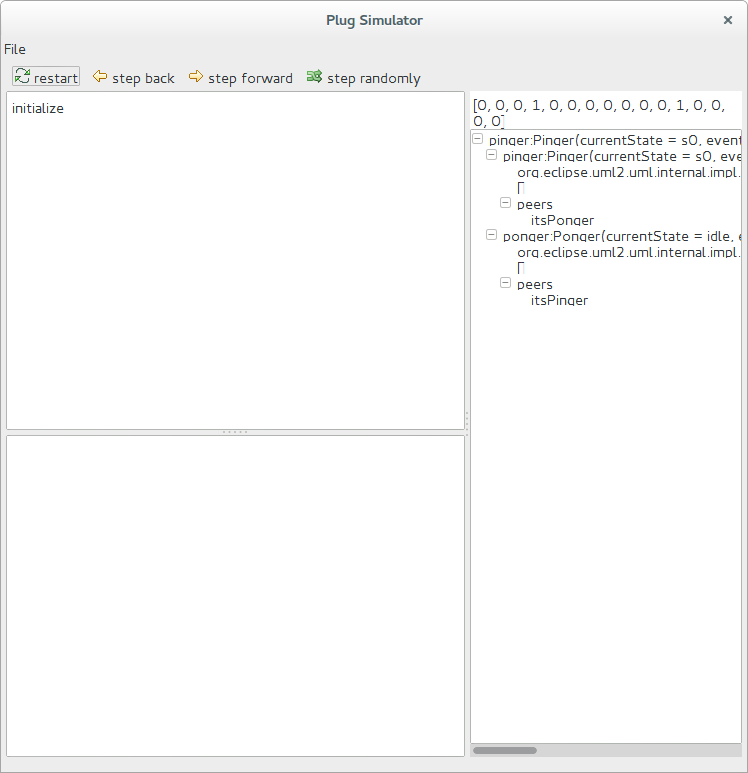
\includegraphics[width=0.5\textwidth]{simulator}
  \caption{Mr Teodorov simulator}
  \label{fig:sim}
\end{figure}


The simulator is compose on 4 part.
\begin{itemize}
\item On the top: some buttons to select an action
\item On the top-left-corner: The list of the next step
\item On the bottom-left-corner: The State Machine associated to the Current State.
\item On the right: A visualization of the Statechart
\end{itemize}







%%% Local Variables:
%%% mode: latex
%%% TeX-master: "../rapport_de_base"
%%% End:
